\documentclass[12pt]{article}
\usepackage{url,graphicx,tabularx,array}
\usepackage[margin=1in]{geometry}
\setlength{\parskip}{1ex} %--skip lines between paragraphs
\setlength{\parindent}{0pt} %--don't indent paragraphs

\usepackage{algorithmic}
\usepackage{algorithm}
\usepackage{ amssymb }
\usepackage{ latexsym }
\usepackage{ amsmath }
\usepackage{ amsthm }
%-- Commands for header
\renewcommand{\title}[1]{\textbf{#1}\\}
\renewcommand{\line}{\begin{tabularx}{\textwidth}{X>{\raggedleft}X}\hline\\\end{tabularx}\\[-0.5cm]}
\newcommand{\leftright}[2]{\begin{tabularx}{\textwidth}{X>{\raggedleft}X}#1%
& #2\\\end{tabularx}\\[-0.5cm]}

\newtheorem{defn}{Definition}[section]
\newtheorem{conjecture}{conjecture}[section]
\newtheorem{lemma}{Lemma}[section]
\newtheorem{corollary}{Corollary}[section]
\newtheorem{question}{Question}[section]
\newtheorem{proposition}{Proposition}[section]


%\linespread{2} %-- Uncomment for Double Space
\begin{document}

\title{Homework 4: CMPS 242}
\line
\leftright{\today}{Bryan Matsuo (bmatsuo@soe.ucsc.edu) \& John St. John (jstjohn@soe.ucsc.edu)} %-- left and right positions in the header
\begin{enumerate}
\item \textbf{Neural Networks:}
Here is the formula for the output at node 5 produced by the network from Figure 1 in the back-propagation handout.
\[
\sigma\left(w_{5,0}+w_{5,3}\sigma\left(w_{3,0}+\sum_{i=1}^2w_{3,i}z_i\right)+w_{5,4}\sigma\left(w_{4,0}+\sum_{i=1}^2w_{4,i}z_i\right) \right)
\]

\item \textbf{Decision Tree:}

Below are the impurity calculations given the choice of each node as root. The root with the lowest impurity is $x_1$ so that is the one that will be chosen.

Root=\[x_1: -\left(1/3\left(1\log_2 1 + 0\log_2 0 \right)+ 2/3 \left( 1/2\log_2 1/2 + 1/2\log_2 1/2\right)\right) = 0.667\]
Root=\[x_2: -\left(2/3\left( 2/3\log_2 2/3 + 1/3\log_2 1/3 \right) + 1/3 \left( 2/3\log_2 2/3 + 1/3\log_2 1/3 \right) \right)= 0.918 \]
Root=\[x_3: -\left(1/3\left( 2/3\log_2 2/3 + 1/3\log_2 1/3\right) + 2/3 \left( 2/3\log_2 2/3 + 1/3\log_2 1/3 \right)\right) =  0.918 \]


\item \textbf{Perceptrion Algorithm:}

\begin{enumerate}
\item \textit{Experiment 1:}

There is a definite relationship between both the number of gaps and the number of mistakes made. Figure~\ref{fig:gvm} clearly shows that the number of mistakes are upper bounded by $\frac{1}{\text{Gaps}^2}$, and decrease as the Gap size increases. Figure~\ref{fig:mvi} shows that the number of iterations required to reach a consistent hypothesis and the number of mistakes eventually made are highly correlated with eachother (Pearson's correlation coefficient of $0.9973$) so examining one variable against the Gap is equivalent to the other.


\begin{figure}[htbp]
\begin{center}
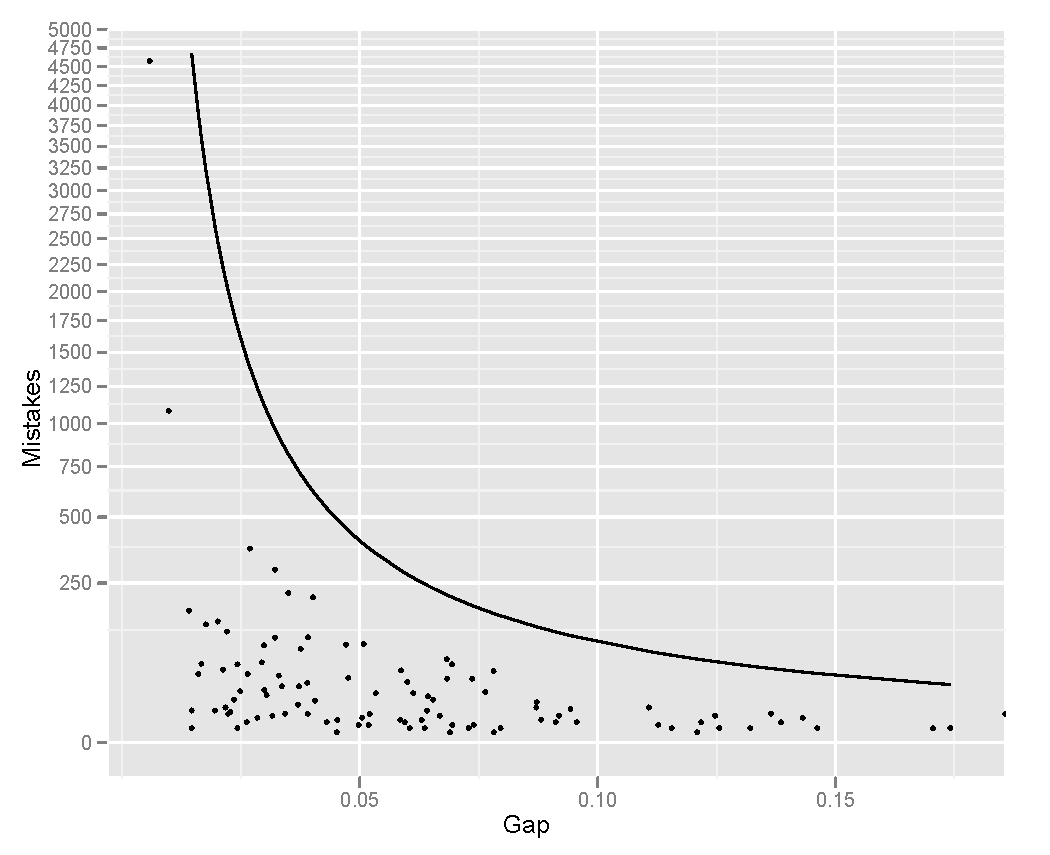
\includegraphics[scale=0.7]{ex1_gap_vs_Mistakes}
\caption{Comparing gaps to the total number of mistakes shows that as the gap increases in size, fewer mistakes are made. Interestingly, all of our points are well within the theoretical upper bound of the number of mistakes made is $\frac{1}{\text{Gap}^2}$}
\label{fig:gvm}
\end{center}

\end{figure}
\begin{figure}[htbp]
\begin{center}
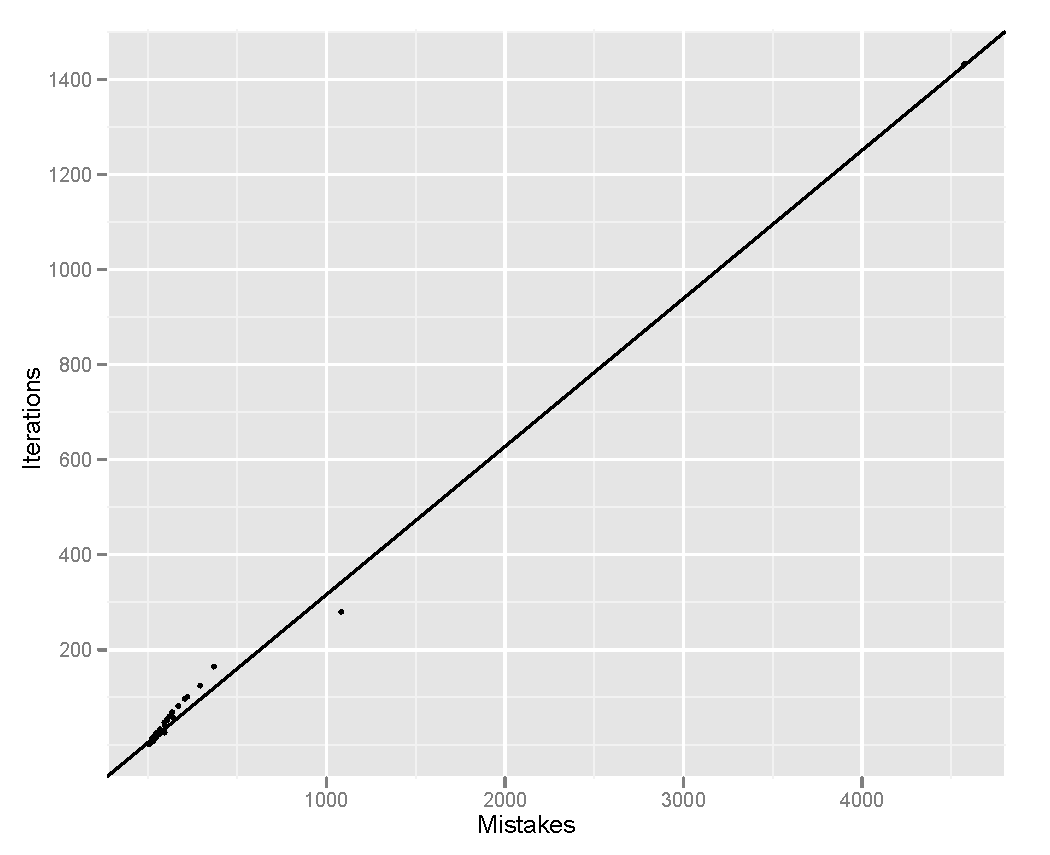
\includegraphics[scale=0.7]{ex1_iteration_mistakes}
\caption{Iterations and Mistakes are highly correlated with a Pearson's correlation coefficient of $0.9973$. Thus you are pretty safe just comparing one of those two values to the Gap as we did in Figure~\ref{fig:gvm}}
\label{fig:mvi}
\end{center}
\end{figure}


\item \textit{Experiment 2:}


\end{enumerate}
\end{enumerate}
\end{document}
